% !TEX root = ../LinalColloc02.tex
\section{Действия над матрицами и их свойства}
\begin{conj}
    Матрица над кольцом $R$ -- прямоугольная таблица, составленная из элементов кольца $R$.
\end{conj}
Задать матрицу $A$ -- задать набор элементов $a_{ij} \in R$ для всех $i, \, j$ таких, что $1 \leq i \leq m, \, 1 \leq j \leq n$.
Эти элементы называются коэффициентами матрицы $A$. Можно писать так: $A = (a_{ij})$. 

Множество всех матриц $m \times n$ над кольцом $R$ обозначается через $M(m, n, R)$.
\begin{conj}
    Квадратная матрица -- матрица, у которой число строк совпадает с числом столбцов.
    Обозначается как $M(n, R)$, где $n$ -- порядок матрицы.
\end{conj}

\underline{Операции над матрицами:}
\begin{enumerate}
    \item Сложение
    \begin{gather*}
        A \in M(m, n, R), \, B \in M(m, n, R) \\
        (A + B)_{ij} = A_{ij} + B_{ij}
    \end{gather*}
    \item Умножение
    \begin{gather*}
        A \in M(m, n, R), \, B \in M(n, p, R) \\
        (AB)_{ik} = \sum_{j = 1}^n A_{ij} B_{jk} 
    \end{gather*}
    \item Умножение на скаляр
    \begin{gather*}
        A \in M(m, n, R), \, \lambda \in R \\
        (\lambda A)_{ij} = \lambda A_{ij}
    \end{gather*}
    \item Транспонирование
    \begin{gather*}
        A \in M(m, n, R), \, A^T \in M(n, m, R) \\
        A^T_{ij} = A_{ji}
    \end{gather*}
\end{enumerate}

\textbf{Теорема} (свойства операций над матрицами).
\textit{
Следующие тождества выполняются для любых матриц $A, B, C$ над коммутативным кольцом $R$ 
и для любых $\lambda, \mu \in R$, если определены результаты всех входящих в них операций:
\begin{enumerate}
    \item $A + (B + C) = (A + B) + C$ 
    \item пусть 0 -- матрица, все коэффициенты которой нулевые; тогда $A + 0 = 0 + A = A$ 
    \item для любой матрицы $A$ найдется матрица $-A$ такая, что $A + (-A) = (-A) + A = 0$
    \item $A + B = B + A$
    \item $A(BC) = (AB)C$
    \item $A(B + C) = AB + AC$
    \item $(B + C)A = BA + CA$
    \item $\lambda (A + B) = \lambda A + \lambda B$
    \item $(\lambda + \mu)A = \lambda A + \mu A$
    \item $(\lambda A)B = \lambda (AB) = A(\lambda B)$
    \item $(\lambda \mu)A = \lambda(\nu A)$
    \item $(A + B)^T = A^T + B^T$
    \item $(AB)^T = B^T A^T$
\end{enumerate}
}
\begin{proof} \quad \\
    Просто скрины конспекта от Жукова.
\end{proof}
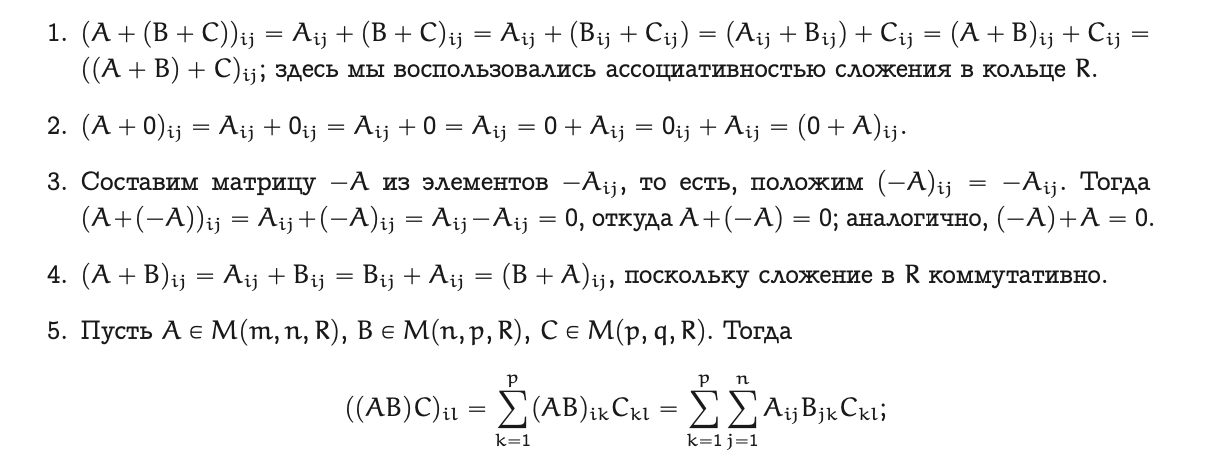
\includegraphics[scale=0.7]{Screenshot1.png} \\
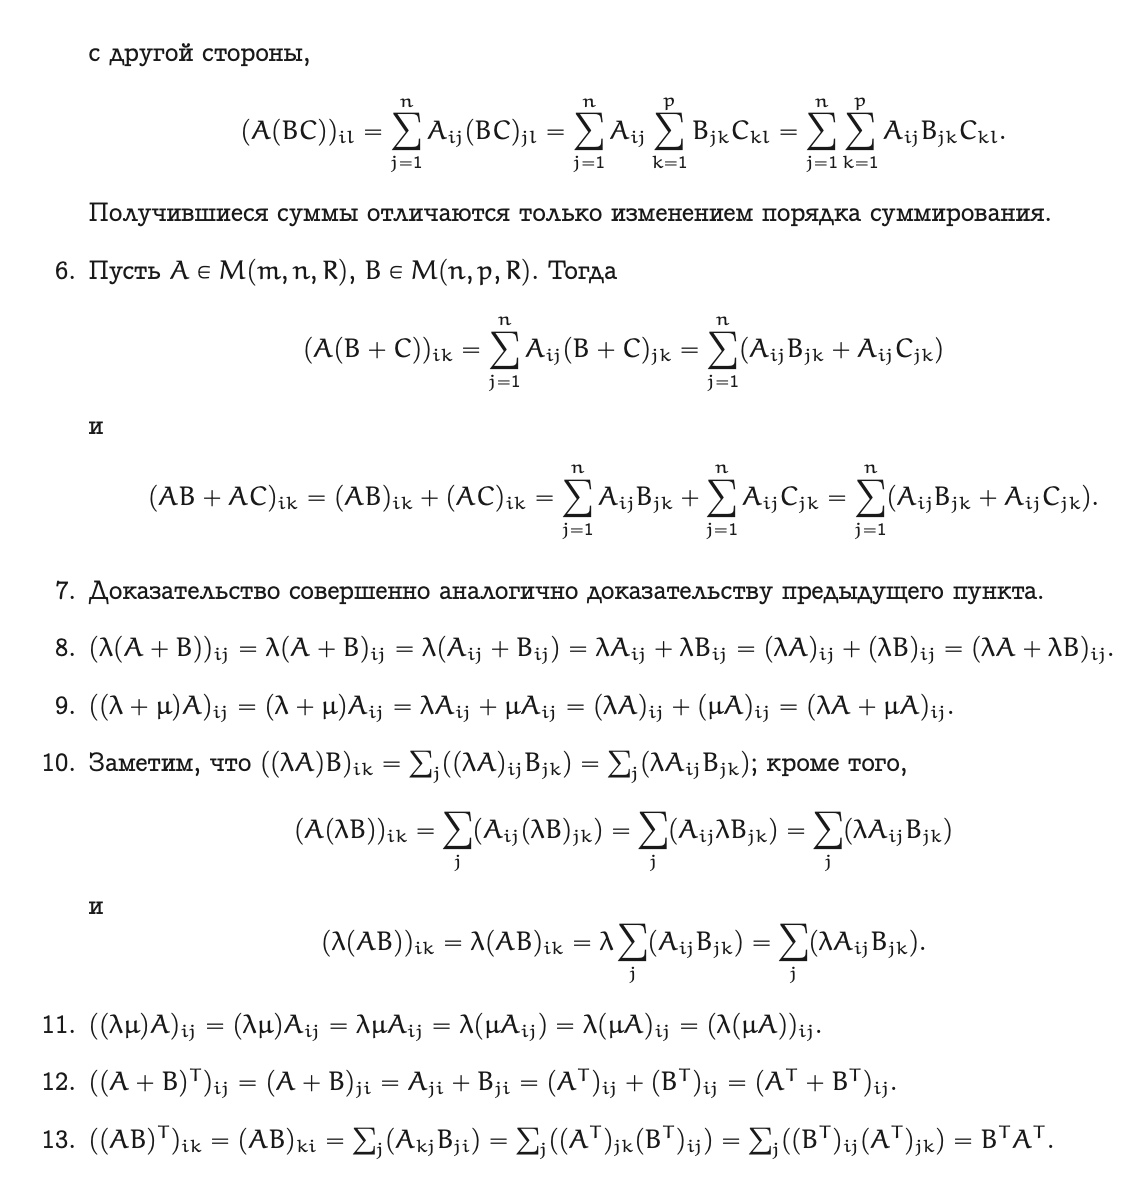
\includegraphics[scale=0.7]{Screenshot2.png}

\begin{conj}
    Единичная матрица -- квадратная матрица, у которой на главной диагонали стоят 1, а на всех остальных позициях 0.
    Обозначается как $E_n$. 
\end{conj}

\begin{theorem-non}
    Пусть $A \in M(m, n, R)$. Тогда $E_m \cdot A = A \cdot E_n = A$.
\end{theorem-non}

\begin{proof}
    $(E_m \cdot A)_{ik} = \sum_{j = 1}^m (E_m)_{ij} A_{jk}$. 
    Заметим, что от суммы останется только одно слагаемое, соответствующее случаю $i = j$, 
    и равное $A_{ik}$. Это выполнено для всех $i, k$, поэтому $E_m \cdot A = A$. 
    Второе равенство доказывается аналогично.
\end{proof}

\begin{follow}
    $M(n, R)$ -- ассоциативное кольцо с 1
\end{follow}

\vspace{7mm}

\begin{conj}
    Квадратная матрица $A \in M(n, R)$ называется обратимой, если найдется матрица $A^{-1} \in M(n, R)$ такая, что $A \cdot A^{-1} = A^{-1} \cdot A = E_n$.
\end{conj}

\begin{notice}
    $M(n, R)^* = GL(n, R)$ (обратимые матрицы образуют группу по умножению)
\end{notice}

\vspace{7mm}

\begin{theorem-non}
    Если матрица $A \in M(n, R)$ обратима, то и матрица $A^T$ обратима, причем $(A^T)^{-1} = (A^{-1})^T$.
\end{theorem-non}

\begin{proof}
    Пользуясь свойством 13 теоремы, доказанной выше, получаем, что $A^T \cdot (A^{-1})^T = (A^{-1} \cdot A)^T = (E_n)^T = E_n$. 
    Равенство $(A^{-1})^T \cdot A^T = E_n$ проверяется аналогично.
\end{proof}